\subsection{Serverless UI}

Another instrumental part of the project is the UI. Without any form of visualisation our whole data
gathering process would not be of much use. For this reason we decided early on what kind of front
end web development stack we would use. Since both us are familiar with \textit{React} - a
\textit{JavaScript} framework famous for revolutionising the use of the \textit{virtual DOM}
to render \textit{UI} elements and to update \textit{UI} elements reactively on
UI change - we decided on using \textit{MarkoJS}.

\subsubsection{MarkoJS}

\textit{MarkoJS} shares many of the same benefits as \textit{React} with some added flexibility like
\textit{concise HTML syntax} which makes the whole \textit{markup} more readable and easier to
write. It also has the ability to use conventional control flow structures like \textit{if} or
\textit{for} directly in the \textit{markup}.

\subsubsection{Babel}

However \textit{MarkoJS} is most and foremost a \textit{JavaScript} framework and due to the nature
of the before mentioned features, \textit{transpiling} is inevitable. \textit{Transpiling} means to
transform modern possibly unsupported \textit{JavaScript} into valid \textit{ECMAScript 5} compliant
code that any browser can understand. For this process we currently use the industry standard
technology \textit{Babel}. With \textit{Babel} \textit{transpiling} is rather easy. All necessary
definitions are in a \textit{webpack.config.babel.js} file which brings us to the next essential
tool \textit{Webpack}.

\subsubsection{Webpack}

“Webpack is a module bundler. Its main purpose is to bundle JavaScript files for usage in a browser,
yet it is also capable of transforming, bundling, or packaging just about any resource or asset.”

With that being said \textit{Webpack} can to some extend be considered as the main part of the whole
\textit{front end stack} as it is responsible for orchestrating \textit{transpiling} of
\textit{MarkoJS} files. It is also responsible for providing \textit{Webpack Dev Server}, a server
that reloads on file change. Furthermore \textit{Webpack} runs all files through certain
optimisation plugins on release build, which can bring down the size of the \textit{code bundle}
quite considerably. \textit{Webpack} is also able to transform \textit{SASS} into \textit{CSS}.

\subsubsection{SASS}

\textit{SASS} is a superset of \textit{CSS} with many additional features like variables, functions,
nesting and exporting/importing files. We make heavy use of those features to structure and
modularise our \textit{CSS} code.

\subsection{UI}

The \textit{UI} itself uses a basic layout where all sensor devices registered in the database are
listed on the side in a so called \textit{sidebar}. The user then can click on each individual
device to open a view with detailed graphs of sensor data of that device. The categories of graphs
are different according to device group. For example \textit{IoT devices} will have different
sensors compared to phones. After a device is selected, the user can then specify the begin and end
time interval according to which sensor data of that device will be filtered and the amount of time
slices. By default the timespan is limited to 24 hours and to 24 time slices. A time slice in our
case is a division of a time interval into equally long time units. To get a single value per time
slice we average all sensor values of a specific sensor between two time slices. Those single values
will then be displayed in the graphs.

\begin{figure}[H]
  \centering
  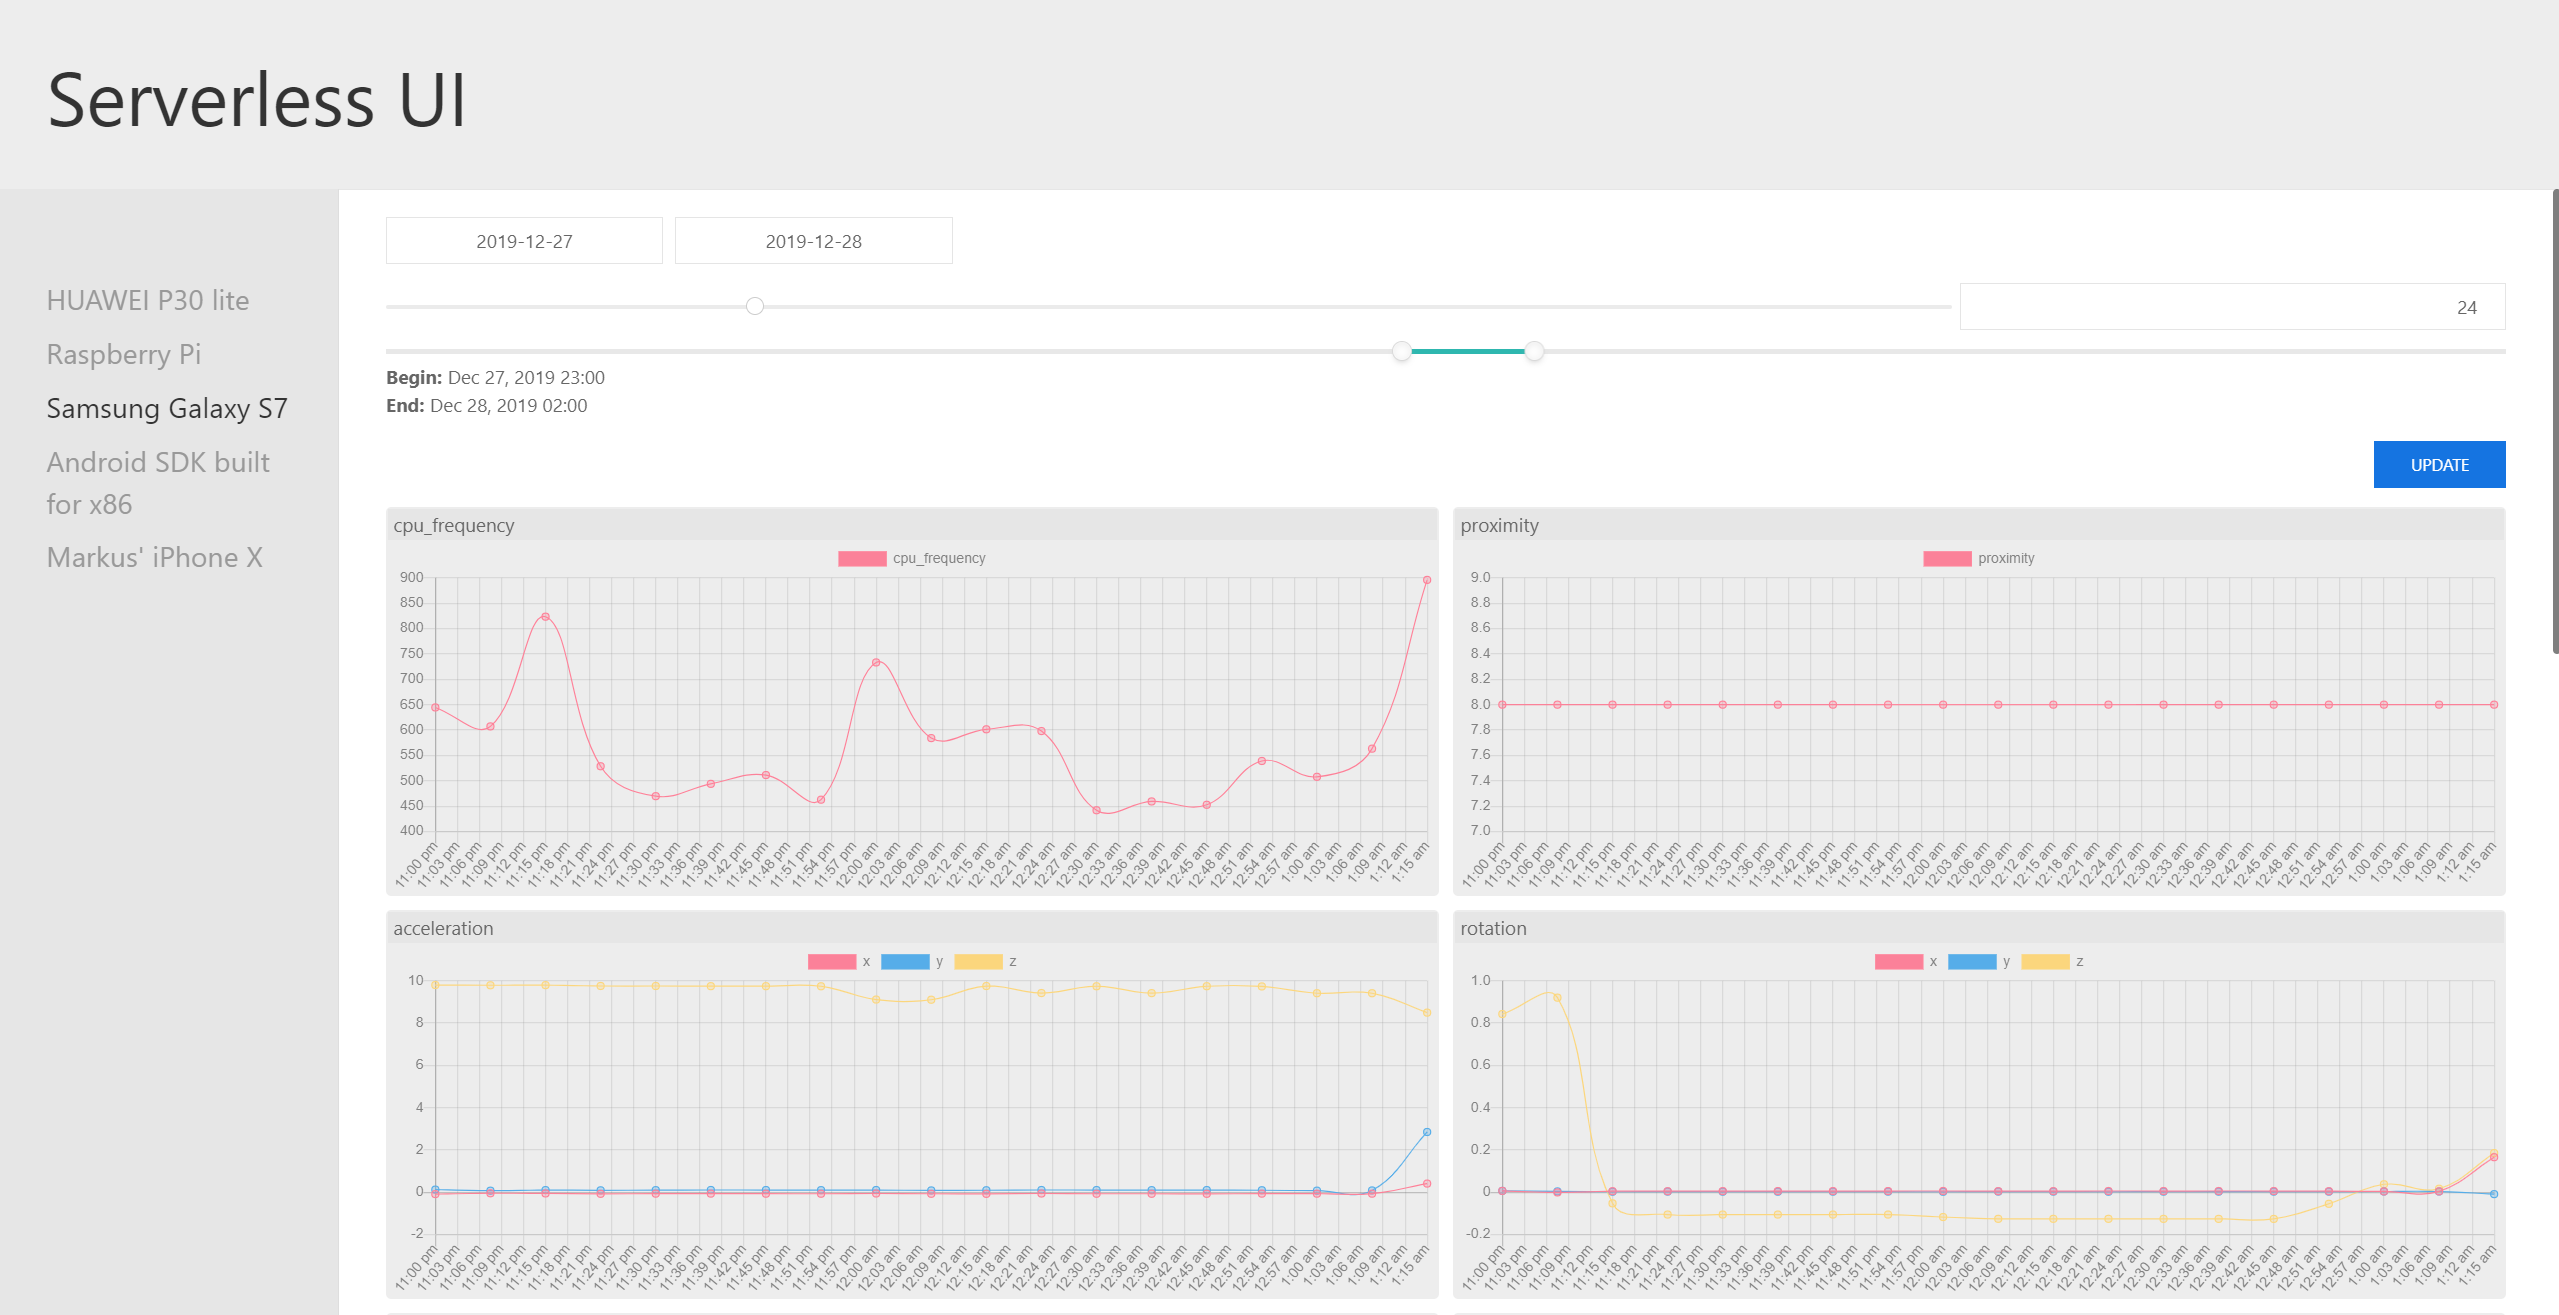
\includegraphics[height=19.5em]{ui-2}
  \caption{Serverless UI - The whole UI: On the left the sidebar can be seen, where all registered devices are listed. In this case the device “Samsung Galaxy S7” is selected and therefore all graphs for this specific device will be shown. }
\end{figure}

\begin{figure}[H]
  \centering
  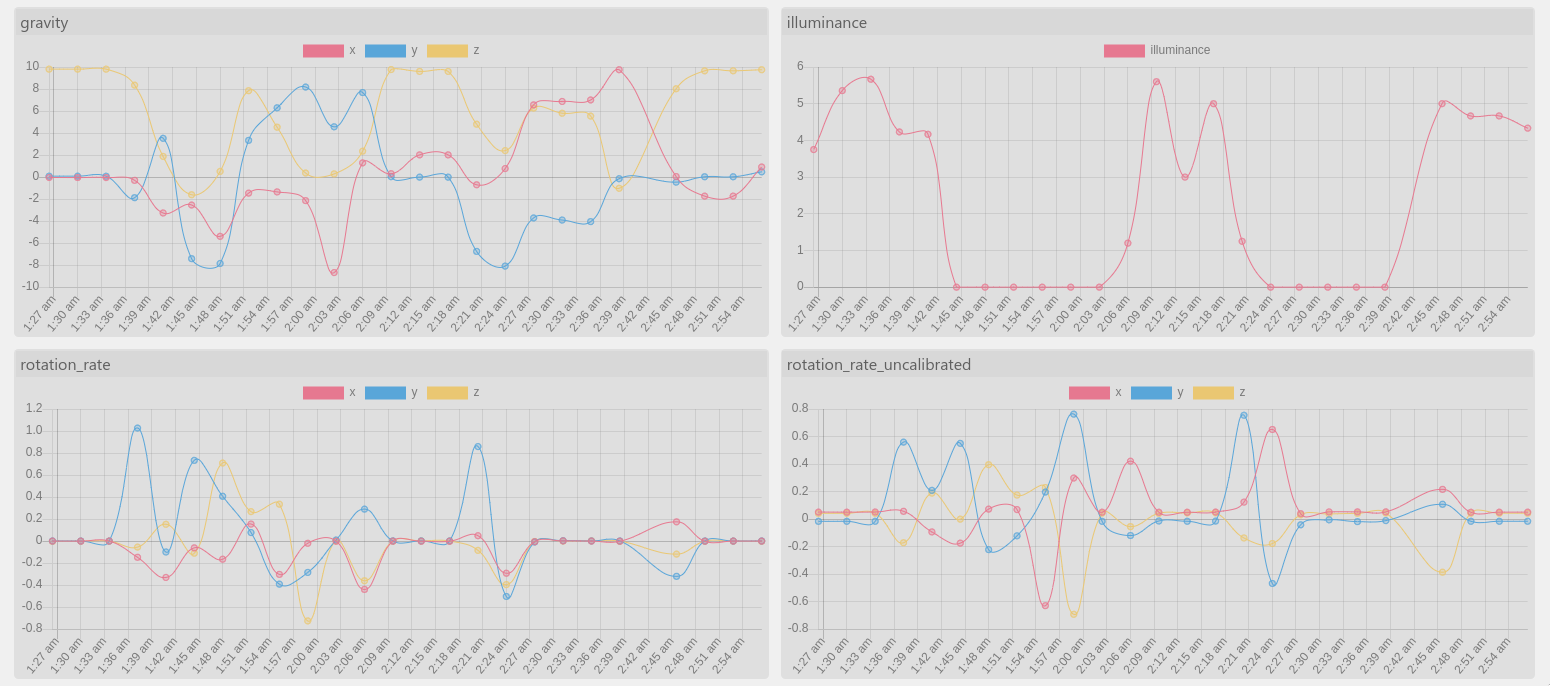
\includegraphics[height=16.5em]{ui-graphs}
  \caption{Serverless UI - Graphs: More graphs for the selected device “Samsung Galaxy S7”.}
\end{figure}

\begin{figure}[H]
  \centering
  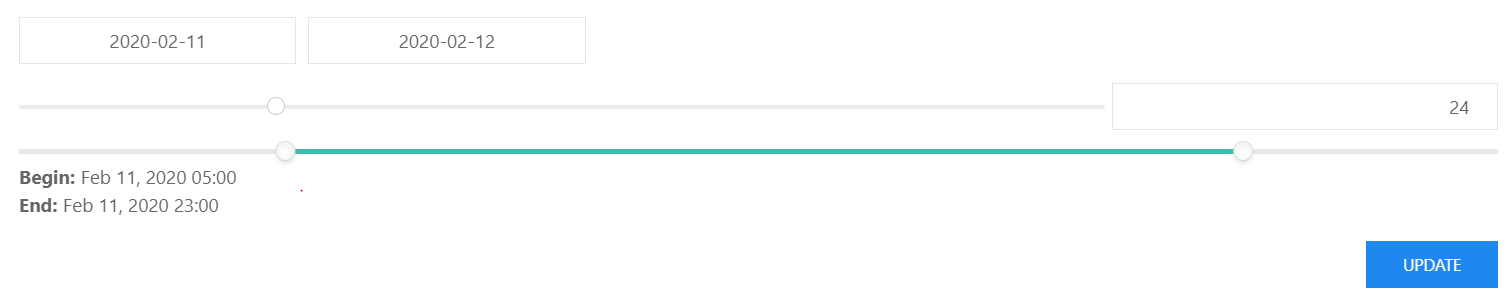
\includegraphics[height=7.5em]{ui-slider}
  \caption{Serverless UI - Slider}
\end{figure}
